\documentclass[10pt,fleqn]{article} % Default font size and left-justified equations
\usepackage[%
    pdftitle={Exercices de SII},
    pdfauthor={Xavier Pessoles}]{hyperref}
\usepackage{afterpage}
\usepackage{subcaption}
\newcommand\blankpage{%
    \null
    \thispagestyle{empty}%
    \addtocounter{page}{-1}%
    \newpage}
    
\newcommand{\repRel}{../..}
\input{\repRel/Style/packages}
%%%%%%%%%%%%%%%%%%%%%%%%%%%%%%%%%%%%%%%%%
% Original author:
% Mathias Legrand (legrand.mathias@gmail.com) with modifications by:
% Vel (vel@latextemplates.com)
% License:
% CC BY-NC-SA 3.0 (http://creativecommons.org/licenses/by-nc-sa/3.0/)
%%%%%%%%%%%%%%%%%%%%%%%%%%%%%%%%%%%%%%%%%

%----------------------------------------------------------------------------------------
%	VARIOUS REQUIRED PACKAGES AND CONFIGURATIONS
%----------------------------------------------------------------------------------------

\usepackage[top=2.5cm,bottom=2cm,left=2cm,right=2cm,headsep=40pt,a4paper]{geometry} % Page margins

\usepackage{graphicx} % Required for including pictures
\graphicspath{{images/}} % Specifies the directory where pictures are stored

\usepackage{lipsum} % Inserts dummy text

\usepackage{tikz} % Required for drawing custom shapes

\usepackage[french]{babel} % English language/hyphenation
\frenchbsetup{StandardLists=true} % Pour éviter la collision babel enumitem pour les listes

\usepackage{enumitem} % Customize lists
\setlist{nolistsep} % Reduce spacing between bullet points and numbered lists

\usepackage{booktabs} % Required for nicer horizontal rules in tables

\usepackage{xcolor} % Required for specifying colors by name
%\definecolor{ocre}{RGB}{243,102,25} % Define the orange color used for highlighting throughout the book
 \definecolor{ocre}{RGB}{49,133,156} % Couleur ''bleue''
\definecolor{violetf}{RGB}{112,48,160} % Couleur ''violet''
\usepackage{enumitem}
\usepackage{pifont} % Pour les dinglist
\usepackage{multicol}
\usepackage{array} % Centrage vertical dans les tableaux

%----------------------------------------------------------------------------------------
%	FONTS
%----------------------------------------------------------------------------------------

\usepackage{avant} % Use the Avantgarde font for headings
%\usepackage{times} % Use the Times font for headings
%\usepackage{mathptmx} % Use the Adobe Times Roman as the default text font together with math symbols from the Sym­bol, Chancery and Com­puter Modern fonts
\usepackage[adobe-utopia]{mathdesign}
\usepackage{microtype} % Slightly tweak font spacing for aesthetics
\usepackage[utf8]{inputenc} % Required for including letters with accents
\usepackage[T1]{fontenc} % Use 8-bit encoding that has 256 glyphs

%----------------------------------------------------------------------------------------
%	BIBLIOGRAPHY AND INDEX
%----------------------------------------------------------------------------------------

\usepackage[style=alphabetic,citestyle=numeric,sorting=nyt,sortcites=true,autopunct=true,babel=hyphen,hyperref=true,abbreviate=false,backref=true,backend=biber]{biblatex}
\addbibresource{bibliography.bib} % BibTeX bibliography file
\defbibheading{bibempty}{}

\usepackage{calc} % For simpler calculation - used for spacing the index letter headings correctly
\usepackage{makeidx} % Required to make an index
\makeindex % Tells LaTeX to create the files required for indexing

%----------------------------------------------------------------------------------------
%	MAIN TABLE OF CONTENTS
%----------------------------------------------------------------------------------------

\usepackage{titletoc} % Required for manipulating the table of contents

\setcounter{tocdepth}{2}     % Dans la table des matieres
\setcounter{secnumdepth}{2}

\contentsmargin{0cm} % Removes the default margin

% Part text styling
\titlecontents{part}[0cm]
{\addvspace{20pt}\centering\large\bfseries}
{}
{}
{}

% Chapter text styling
\titlecontents{chapter}[1.25cm] % Indentation
{\addvspace{12pt}\large\sffamily\bfseries} % Spacing and font options for chapters
{\color{ocre!60}\contentslabel[\Large\thecontentslabel]{1.25cm}\color{ocre}} % Chapter number
{\color{ocre}}  
{\color{ocre!60}\normalsize\;\titlerule*[.5pc]{.}\;\thecontentspage} % Page number

% Section text styling
\titlecontents{section}[1.25cm] % Indentation
{\addvspace{3pt}\sffamily\bfseries} % Spacing and font options for sections
{\color{ocre!60}\contentslabel[\thecontentslabel]{1.25cm} \color{ocre}} % Section number
{\color{ocre}}
{\hfill\color{ocre!60}\thecontentspage} % Page number
[]

% Subsection text styling
\titlecontents{subsection}[1.25cm] % Indentation
{\addvspace{1pt}\sffamily\small} % Spacing and font options for subsections
{\contentslabel[\thecontentslabel]{1.25cm}} % Subsection number
{}
{\ \titlerule*[.5pc]{.}\;\thecontentspage} % Page number
[]


% Subsection text styling
\titlecontents{subsubsection}[1.25cm] % Indentation
{\addvspace{1pt}\sffamily\small} % Spacing and font options for subsections
{\contentslabel[\thecontentslabel]{1.25cm}} % Subsection number
{}
{\ \titlerule*[.5pc]{.}\;\thecontentspage} % Page number
[]

% List of figures
\titlecontents{figure}[0em]
{\addvspace{-5pt}\sffamily}
{\thecontentslabel\hspace*{1em}}
{}
{\ \titlerule*[.5pc]{.}\;\thecontentspage}
[]

% List of tables
\titlecontents{table}[0em]
{\addvspace{-5pt}\sffamily}
{\thecontentslabel\hspace*{1em}}
{}
{\ \titlerule*[.5pc]{.}\;\thecontentspage}
[]

%----------------------------------------------------------------------------------------
%	MINI TABLE OF CONTENTS IN PART HEADS
%----------------------------------------------------------------------------------------

% Chapter text styling
\titlecontents{lchapter}[0em] % Indenting
{\addvspace{15pt}\large\sffamily\bfseries} % Spacing and font options for chapters
{\color{ocre}\contentslabel[\Large\thecontentslabel]{1.25cm}\color{ocre}} % Chapter number
{}  
{\color{ocre}\normalsize\sffamily\bfseries\;\titlerule*[.5pc]{.}\;\thecontentspage} % Page number

% Section text styling
\titlecontents{lsection}[0em] % Indenting
{\sffamily\small} % Spacing and font options for sections
{\contentslabel[\thecontentslabel]{1.25cm}} % Section number
{}
{}

% Subsection text styling
\titlecontents{lsubsection}[.5em] % Indentation
{\normalfont\footnotesize\sffamily} % Font settings
{}
{}
{}

%----------------------------------------------------------------------------------------
%	PAGE HEADERS
%----------------------------------------------------------------------------------------

\usepackage{fancyhdr} % Required for header and footer configuration



\pagestyle{fancy}
 \renewcommand{\headrulewidth}{0pt}
 \fancyhead{}
 \fancyhead[L]{%
 \noindent\begin{minipage}[c]{2.6cm}%
 
\includegraphics[width=2cm]{png/logo_upsti.png}%
 \end{minipage}}

\fancyhead[C]{\rule{8cm}{.5pt}}

 \fancyhead[R]{%
 \noindent\begin{minipage}[c]{3cm}
 \begin{flushright}
 \footnotesize{\textit{\textsf{\xxtete}}}%
 \end{flushright}
 \end{minipage}
}


\fancyfoot[C]{\rule{12cm}{.5pt}}
\renewcommand{\footrulewidth}{0.2pt}
\fancyfoot[C]{\footnotesize{\bfseries \thepage}}
\fancyfoot[L]{ 
\begin{minipage}[c]{.4\linewidth}
\noindent\footnotesize{{\xxauteur}}
\end{minipage}}


\fancyfoot[R]{\footnotesize{\xxpied}
\ifthenelse{\isodd{\value{page}}}{
\begin{tikzpicture}[overlay]
\node[shape=rectangle, 
      rounded corners = .25 cm,
	  draw= ocre,
	  line width=2pt, 
	  fill = ocre!10,
	  minimum width  = 2.5cm,
	  minimum height = 3cm,] at (\xxposongletx,\xxposonglety) {};
\node at (\xxposonglettext,\xxposonglety) {\rotatebox{90}{\textbf{\large\color{ocre}{\xxonglet}}}};
%{};
\end{tikzpicture}}{}
}
%
%
%
% Removes the header from odd empty pages at the end of chapters
\makeatletter
\renewcommand{\cleardoublepage}{
\clearpage\ifodd\c@page\else
\hbox{}
\vspace*{\fill}
\thispagestyle{empty}
\newpage
\fi}

\fancypagestyle{plain}{%
\fancyhf{} % vide l’en-tête et le pied~de~page.
%\fancyfoot[C]{\bfseries \thepage} % numéro de la page en cours en gras
% et centré en pied~de~page.
\fancyfoot[R]{\footnotesize{\xxpied}}
\fancyfoot[C]{\rule{12cm}{.5pt}}
\renewcommand{\footrulewidth}{0.2pt}
\fancyfoot[C]{\footnotesize{\bfseries \thepage}}
\fancyfoot[L]{ 
\begin{minipage}[c]{.4\linewidth}
\noindent\footnotesize{{\xxauteur}}
\end{minipage}}}



%----------------------------------------------------------------------------------------
%	THEOREM STYLES
%----------------------------------------------------------------------------------------

% Conflit avec la police adobe
%\usepackage{amsmath,amsfonts,amssymb,amsthm} % For math equations, theorems, symbols, etc
\usepackage{amsmath,amsthm}

\newcommand{\intoo}[2]{\mathopen{]}#1\,;#2\mathclose{[}}
\newcommand{\ud}{\mathop{\mathrm{{}d}}\mathopen{}}
\newcommand{\intff}[2]{\mathopen{[}#1\,;#2\mathclose{]}}
%\newtheorem{notation}{Notation}[chapter]
\newtheorem{notation}{Notation}[section]

% Boxed/framed environments
\newtheoremstyle{ocrenumbox}% % Theorem style name
{0pt}% Space above
{0pt}% Space below
{\normalfont}% % Body font
{}% Indent amount
{\small\bf\sffamily\color{ocre}}% % Theorem head font
{\;}% Punctuation after theorem head
{0.25em}% Space after theorem head
{\small\sffamily\color{ocre}\thmname{#1}\nobreakspace\thmnumber%{\@ifnotempty{#1}{}\@upn{#2}}% Theorem text (e.g. Theorem 2.1)
\thmnote{\nobreakspace\the\thm@notefont\sffamily\bfseries\color{black}---\nobreakspace#3.}} % Optional theorem note
\renewcommand{\qedsymbol}{$\blacksquare$}% Optional qed square


% Boite pour les corriges
\newtheoremstyle{correctionbox}% % Theorem style name
{0pt}% Space above
{0pt}% Space below
{\normalfont}% % Body font
{}% Indent amount
{\small\bf\sffamily\color{violet}}% % Theorem head font
{\;}% Punctuation after theorem head
{0.25em}% Space after theorem head
{\small\sffamily\color{ocre}\thmname{#1}\nobreakspace\thmnumber%{\@ifnotempty{#1}{}\@upn{#2}}% Theorem text (e.g. Theorem 2.1)
\thmnote{\nobreakspace\the\thm@notefont\sffamily\bfseries\color{black}---\nobreakspace#3.}} % Optional theorem note
\renewcommand{\qedsymbol}{$\blacksquare$}% Optional qed square



\newtheoremstyle{blacknumex}% Theorem style name
{5pt}% Space above
{5pt}% Space below
{\normalfont}% Body font
{} % Indent amount
{\small\bf\sffamily}% Theorem head font
{\;}% Punctuation after theorem head
{0.25em}% Space after theorem head
{\small\sffamily{\tiny\ensuremath{\blacksquare}}\nobreakspace\thmname{#1}\nobreakspace\thmnumber%{\@ifnotempty{#1}{}\@upn{#2}}% Theorem text (e.g. Theorem 2.1)
\thmnote{\nobreakspace\the\thm@notefont\sffamily\bfseries---\nobreakspace#3.}}% Optional theorem note

\newtheoremstyle{blacknumbox} % Theorem style name
{0pt}% Space above
{0pt}% Space below
{\normalfont}% Body font
{}% Indent amount
{\small\bf\sffamily}% Theorem head font
{\;}% Punctuation after theorem head
{0.25em}% Space after theorem head
{\small\sffamily\thmname{#1}\nobreakspace 
\thmnote{\nobreakspace\the\thm@notefont\sffamily\bfseries---\nobreakspace#3.}}% Optional theorem note

% Non-boxed/non-framed environments
\newtheoremstyle{ocrenum}% % Theorem style name
{5pt}% Space above
{5pt}% Space below
{\normalfont}% % Body font
{}% Indent amount
{\small\bf\sffamily\color{ocre}}% % Theorem head font
{\;}% Punctuation after theorem head
{0.25em}% Space after theorem head
{\small\sffamily\color{ocre}\thmname{#1}\nobreakspace%\thmnumber{\@ifnotempty{#1}{}\@upn{#2}}% Theorem text (e.g. Theorem 2.1)
\thmnote{\nobreakspace\the\thm@notefont\sffamily\bfseries\color{black}---\nobreakspace#3.}} % Optional theorem note
\renewcommand{\qedsymbol}{$\blacksquare$}% Optional qed square
\makeatother

% Environnement pour les titres de parties
\newtheoremstyle{partiebox} 
{0pt}% Space above
{0pt}% Space below
{\normalfont}% Body font
{}% Indent amount
{\small\bf\sffamily}% Theorem head font
{\;}% Punctuation after theorem head
{0.25em}% Space after theorem head




% Defines the theorem text style for each type of theorem to one of the three styles above
\newcounter{dummy} 
\numberwithin{dummy}{section}
\theoremstyle{ocrenumbox}
%\newtheorem{theoremeT}[dummy]{Théorème}
\newtheorem{theoremeT}[dummy]{Théorème}
\newtheorem{resultatT}[dummy]{Résultat}
\newtheorem{savoirT}[dummy]{Savoir}
\newtheorem{methodeT}[dummy]{Méthode}
\newtheorem{objectifT}[dummy]{Objectif}
%\newtheorem{problem}{Problem}[chapter]
\newtheorem{problem}{Problem}[section]
%\newtheorem{exerciseT}{Exercise}[chapter]
\newtheorem{exerciseT}{Exercice}[section]

\theoremstyle{blacknumex}
%\newtheorem{exampleT}{Example}[chapter]
\newtheorem{exempleT}{Exemple}[section]
\newtheorem{termT}{Terminal\\}[section]
\newtheorem{pyT}{Python\\}[section]
\newtheorem{sciT}{Scilab\\}[section]
\newtheorem{pseudoT}{Pseudo Code\\}[section]
\newtheorem{sqlT}{SQL\\}[section]

\theoremstyle{blacknumbox}
%\newtheorem{vocabulary}{Vocabulary}[chapter]
\newtheorem{vocabulary}{Vocabulaire}[section]
%\newtheorem{definitionT}{Definition}[section]
\newtheorem{definitionT}{Définition}[section]
\newtheorem{rappelT}{Rappel}[section]
\newtheorem{demoT}{Démonstration}[section]
\newtheorem{corollaryT}[dummy]{Corollaire}
\newtheorem{hypoT}{Hypothèse(s)}

\theoremstyle{ocrenum}
\newtheorem{proposition}[dummy]{Proposition}

\theoremstyle{partiebox}
\newtheorem{titrepartieT}[]{}
\newtheorem{titrechapitreT}[]{}

\theoremstyle{correctionbox}
\newtheorem{correctionT}[dummy]{\color{violet}{Correction}}

%----------------------------------------------------------------------------------------
%	DEFINITION OF COLORED BOXES
%----------------------------------------------------------------------------------------

\RequirePackage[framemethod=tikz]{mdframed} % Required for creating the theorem, definition, exercise and corollary boxes

% Theorem box
\newmdenv[skipabove=7pt,
skipbelow=7pt,
backgroundcolor=ocre!10,
linecolor=ocre,
innerleftmargin=5pt,
innerrightmargin=5pt,
innertopmargin=5pt,
leftmargin=0cm,
rightmargin=0cm,
innerbottommargin=5pt]{tBox}


% Correction
\newmdenv[skipabove=7pt,
skipbelow=7pt,
backgroundcolor=violet!10,
linecolor=violet,
innerleftmargin=5pt,
innerrightmargin=5pt,
innertopmargin=5pt,
leftmargin=0cm,
rightmargin=0cm,
innerbottommargin=5pt]{coBox}


% Exercise box	  
\newmdenv[skipabove=7pt,
skipbelow=7pt,
rightline=false,
leftline=true,
topline=false,
bottomline=false,
backgroundcolor=ocre!10,
linecolor=ocre,
innerleftmargin=5pt,
innerrightmargin=5pt,
innertopmargin=5pt,
innerbottommargin=5pt,
leftmargin=0cm,
rightmargin=0cm,
linewidth=4pt]{eBox}	

% Definition box
\newmdenv[skipabove=7pt,
skipbelow=7pt,
rightline=false,
leftline=true,
topline=false,
bottomline=false,
backgroundcolor=ocre!10,
linecolor=ocre,
innerleftmargin=5pt,
innerrightmargin=5pt,
innertopmargin=0pt,
leftmargin=0cm,
rightmargin=0cm,
linewidth=4pt,
innerbottommargin=0pt]{dBox}	

% Demonstration box
\newmdenv[skipabove=7pt,
skipbelow=7pt,
rightline=false,
leftline=true,
topline=false,
bottomline=false,
%backgroundcolor=ocre!10,
linecolor=ocre,
innerleftmargin=5pt,
innerrightmargin=5pt,
innertopmargin=0pt,
leftmargin=0cm,
rightmargin=0cm,
linewidth=4pt,
innerbottommargin=0pt]{demoBox}	

% Corollary box
\newmdenv[skipabove=7pt,
skipbelow=7pt,
rightline=false,
leftline=true,
topline=false,
bottomline=false,
linecolor=gray,
backgroundcolor=black!5,
innerleftmargin=5pt,
innerrightmargin=5pt,
innertopmargin=5pt,
leftmargin=0cm,
rightmargin=0cm,
linewidth=4pt,
innerbottommargin=5pt]{cBox}


% Hypothèses
\newmdenv[skipabove=7pt,
skipbelow=7pt,
rightline=false,
leftline=true,
topline=false,
bottomline=false,
linecolor=gray,
backgroundcolor=black!5,
innerleftmargin=5pt,
innerrightmargin=5pt,
innertopmargin=5pt,
leftmargin=0cm,
rightmargin=0cm,
linewidth=4pt,
innerbottommargin=5pt]{hyBox}


% Boite pour le titre de la partie (pBox)
\newmdenv[skipabove=7pt,
skipbelow=7pt,
rightline=true,
leftline=false,
topline=false,
bottomline=false,
linecolor=ocre,
backgroundcolor=none,
innerleftmargin=5pt,
innerrightmargin=5pt,
innertopmargin=5pt,
leftmargin=0cm,
rightmargin=0cm,
linewidth=4pt,
innerbottommargin=5pt]{pBox}

% Boite pour le titre du chapitre (chBox)
\newmdenv[skipabove=7pt,
skipbelow=7pt,
rightline=false,
leftline=true,
topline=false,
bottomline=false,
linecolor=ocre,
%backgroundcolor=black!5,
innerleftmargin=5pt,
innerrightmargin=5pt,
innertopmargin=5pt,
leftmargin=0cm,
rightmargin=0cm,
linewidth=4pt,
innerbottommargin=5pt]{chBox}


% Boite pour les exemples
\newmdenv[skipabove=7pt,
skipbelow=7pt,
rightline=false,
leftline=true,
topline=false,
bottomline=false,
linecolor=gray,
backgroundcolor=white,
innerleftmargin=5pt,
innerrightmargin=5pt,
innertopmargin=5pt,
leftmargin=0cm,
rightmargin=0cm,
linewidth=4pt,
innerbottommargin=5pt]{exBox}

% Boite pour le terminal
\newmdenv[skipabove=7pt,
skipbelow=7pt,
rightline=false,
leftline=true,
topline=false,
bottomline=false,
linecolor=gray,
backgroundcolor=white,
innerleftmargin=5pt,
innerrightmargin=5pt,
innertopmargin=5pt,
leftmargin=0cm,
rightmargin=0cm,
linewidth=4pt,
innerbottommargin=5pt]{termBox}


% Boite pour Python
\newmdenv[skipabove=7pt,
skipbelow=7pt,
rightline=false,
leftline=true,
topline=false,
bottomline=false,
linecolor=gray,
backgroundcolor=white,
innerleftmargin=5pt,
innerrightmargin=5pt,
innertopmargin=0pt,
leftmargin=0cm,
rightmargin=0cm,
linewidth=4pt,
innerbottommargin=5pt]{pyBox}

% Boite pour scilab
\newmdenv[skipabove=7pt,
skipbelow=7pt,
rightline=false,
leftline=true,
topline=false,
bottomline=false,
linecolor=gray,
backgroundcolor=white,
innerleftmargin=5pt,
innerrightmargin=5pt,
innertopmargin=5pt,
leftmargin=0cm,
rightmargin=0cm,
linewidth=4pt,
innerbottommargin=5pt]{sciBox}


% Boite pour pseudo
\newmdenv[skipabove=7pt,
skipbelow=7pt,
rightline=false,
leftline=true,
topline=false,
bottomline=false,
linecolor=gray,
backgroundcolor=white,
innerleftmargin=5pt,
innerrightmargin=5pt,
innertopmargin=5pt,
leftmargin=0cm,
rightmargin=0cm,
linewidth=4pt,
innerbottommargin=5pt]{pseudoBox}

% Boite pour pseudo
\newmdenv[skipabove=7pt,
skipbelow=7pt,
rightline=false,
leftline=true,
topline=false,
bottomline=false,
linecolor=gray,
backgroundcolor=white,
innerleftmargin=5pt,
innerrightmargin=5pt,
innertopmargin=5pt,
leftmargin=0cm,
rightmargin=0cm,
linewidth=4pt,
innerbottommargin=5pt]{sqlBox}


% Creates an environment for each type of theorem and assigns it a theorem text style from the "Theorem Styles" section above and a colored box from above
\newenvironment{theorem}{\begin{tBox}\begin{theoremeT}}{\end{theoremeT}\end{tBox}}
\newenvironment{resultat}{\begin{tBox}\begin{resultatT}}{\end{resultatT}\end{tBox}}
\newenvironment{methode}{\begin{tBox}\begin{methodeT}}{\end{methodeT}\end{tBox}}
\newenvironment{savoir}{\begin{tBox}\begin{savoirT}}{\end{savoirT}\end{tBox}}
\newenvironment{obj}{\begin{tBox}\begin{objectifT}}{\end{objectifT}\end{tBox}}
\newenvironment{corrige}{\begin{coBox}\begin{correctionT}}{\end{correctionT}\end{coBox}}
\newenvironment{exercise}{\begin{eBox}\begin{exerciseT}}{\hfill{\color{ocre}\tiny\ensuremath{\blacksquare}}\end{exerciseT}\end{eBox}}				  
\newenvironment{exercice}{\begin{eBox}\begin{exerciseT}}{\hfill{\color{ocre}\tiny\ensuremath{\blacksquare}}\end{exerciseT}\end{eBox}}				  

\newenvironment{definition}{\begin{dBox}\begin{definitionT}}{\end{definitionT}\end{dBox}}	
\newenvironment{rappel}{\begin{dBox}\begin{rappelT}}{\end{rappelT}\end{dBox}}	
\newenvironment{defi}{\begin{dBox}\begin{definitionT}}{\end{definitionT}\end{dBox}}	
\newenvironment{demo}{\begin{demoBox}\begin{demoT}}{\end{demoT}\end{demoBox}}	
%\newenvironment{exemple}{\begin{exempleT}}{\hfill{\tiny\ensuremath{\blacksquare}}\end{exempleT}}		
\newenvironment{corollary}{\begin{cBox}\begin{corollaryT}}{\end{corollaryT}\end{cBox}}
\newenvironment{hypo}{\begin{hyBox}\begin{hypoT}}{\end{hypoT}\end{hyBox}}	\newenvironment{exemple}{\begin{exBox}\begin{exempleT}}{\hfill{\tiny\ensuremath{\blacksquare}}\end{exempleT}\end{exBox}}	
\newenvironment{titrepartie}{\begin{pBox}\begin{titrepartieT}}{\end{titrepartieT}\end{pBox}}	
\newenvironment{titrechapitre}{\begin{chBox}\begin{titrechapitreT}}{\end{titrechapitreT}\end{chBox}}	

\newenvironment{term}{ \begin{termBox}\begin{termT}}{\end{termT}\end{termBox}}
\newenvironment{py}{ \begin{pyBox}\begin{pyT}}{\end{pyT}\end{pyBox}}
\newenvironment{sci}{ \begin{sciBox}\begin{sciT}}{\end{sciT}\end{sciBox}}
\newenvironment{pseudo}{ \begin{pseudoBox}\begin{pseudoT}}{\end{pseudoT}\end{pseudoBox}}
\newenvironment{envsql}{ \begin{sqlBox}\begin{sqlT}}{\end{sqlT}\end{sqlBox}}


%----------------------------------------------------------------------------------------
%	REMARK ENVIRONMENT
%----------------------------------------------------------------------------------------

\newenvironment{remark}{\par\vspace{10pt}\small % Vertical white space above the remark and smaller font size
\begin{list}{}{
\leftmargin=35pt % Indentation on the left
\rightmargin=25pt}\item\ignorespaces % Indentation on the right
\makebox[-2.5pt]{\begin{tikzpicture}[overlay]
\node[draw=ocre!60,line width=1pt,circle,fill=ocre!25,font=\sffamily\bfseries,inner sep=2pt,outer sep=0pt] at (-15pt,0pt){\textcolor{ocre}{R}};\end{tikzpicture}} % Orange R in a circle
\advance\baselineskip -1pt}{\end{list}\vskip5pt} % Tighter line spacing and white space after remark

\newenvironment{rem}{\par\vspace{10pt}\small % Vertical white space above the remark and smaller font size
\begin{list}{}{
\leftmargin=35pt % Indentation on the left
\rightmargin=25pt}\item\ignorespaces % Indentation on the right
\makebox[-2.5pt]{\begin{tikzpicture}[overlay]
\node[draw=ocre!60,line width=1pt,circle,fill=ocre!25,font=\sffamily\bfseries,inner sep=2pt,outer sep=0pt] at (-15pt,0pt){\textcolor{ocre}{R}};\end{tikzpicture}} % Orange R in a circle
\advance\baselineskip -1pt}{\end{list}\vskip5pt} % Tighter line spacing and white space after remark


\newenvironment{warn}{\par\vspace{10pt}\small % Vertical white space above the remark and smaller font size
\begin{list}{}{
\leftmargin=35pt % Indentation on the left
\rightmargin=25pt}\item\ignorespaces % Indentation on the right
\makebox[-2.5pt]{\begin{tikzpicture}[overlay]
\node[draw=red!60,line width=1pt,circle,fill=red!25,font=\sffamily\bfseries,inner sep=2pt,outer sep=0pt] at (-15pt,0pt){\textcolor{black}{!}};\end{tikzpicture}} % Point d'exclamation dans un cercle
\advance\baselineskip -1pt}{\end{list}\vskip5pt} % Tighter line spacing and white space after remark


%----------------------------------------------------------------------------------------
%	SECTION NUMBERING IN THE MARGIN
%----------------------------------------------------------------------------------------
\setcounter{secnumdepth}{3}
\setcounter{tocdepth}{2}



\makeatletter
\renewcommand{\@seccntformat}[1]{\llap{\textcolor{ocre}{\csname the#1\endcsname}\hspace{1em}}}                    
\renewcommand{\section}{\@startsection{section}{1}{\z@}
{-4ex \@plus -1ex \@minus -.4ex}
{1ex \@plus.2ex }
{\normalfont\large\sffamily\bfseries}}
\renewcommand{\subsection}{\@startsection {subsection}{2}{\z@}
{-3ex \@plus -0.1ex \@minus -.4ex}
{0.5ex \@plus.2ex }
{\normalfont\sffamily\bfseries}}
\renewcommand{\subsubsection}{\@startsection {subsubsection}{3}{\z@}
{-2ex \@plus -0.1ex \@minus -.2ex}
{.2ex \@plus.2ex }
{\normalfont\small\sffamily\bfseries}}                        
\renewcommand\paragraph{\@startsection{paragraph}{4}{\z@}
{-2ex \@plus-.2ex \@minus .2ex}
{.1ex}
{\normalfont\small\sffamily\bfseries}}

%----------------------------------------------------------------------------------------
%	PART HEADINGS
%----------------------------------------------------------------------------------------


%----------------------------------------------------------------------------------------
%	CHAPTER HEADINGS
%----------------------------------------------------------------------------------------

% \newcommand{\thechapterimage}{}%
% \newcommand{\chapterimage}[1]{\renewcommand{\thechapterimage}{#1}}%
% \def\@makechapterhead#1{%
% {\parindent \z@ \raggedright \normalfont
% \ifnum \c@secnumdepth >\m@ne
% \if@mainmatter
% \begin{tikzpicture}[remember picture,overlay]
% \node at (current page.north west)
% {\begin{tikzpicture}[remember picture,overlay]
% \node[anchor=north west,inner sep=0pt] at (0,0) {\includegraphics[width=\paperwidth]{\thechapterimage}};
% \draw[anchor=west] (\Gm@lmargin,-9cm) node [line width=2pt,rounded corners=15pt,draw=ocre,fill=white,fill opacity=0.5,inner sep=15pt]{\strut\makebox[22cm]{}};
% \draw[anchor=west] (\Gm@lmargin+.3cm,-9cm) node {\huge\sffamily\bfseries\color{black}\thechapter. #1\strut};
% \end{tikzpicture}};
% \end{tikzpicture}
% \else
% \begin{tikzpicture}[remember picture,overlay]
% \node at (current page.north west)
% {\begin{tikzpicture}[remember picture,overlay]
% \node[anchor=north west,inner sep=0pt] at (0,0) {\includegraphics[width=\paperwidth]{\thechapterimage}};
% \draw[anchor=west] (\Gm@lmargin,-9cm) node [line width=2pt,rounded corners=15pt,draw=ocre,fill=white,fill opacity=0.5,inner sep=15pt]{\strut\makebox[22cm]{}};
% \draw[anchor=west] (\Gm@lmargin+.3cm,-9cm) node {\huge\sffamily\bfseries\color{black}#1\strut};
% \end{tikzpicture}};
% \end{tikzpicture}
% \fi\fi\par\vspace*{270\p@}}}

%-------------------------------------------

\def\@makeschapterhead#1{%
\begin{tikzpicture}[remember picture,overlay]
\node at (current page.north west)
{\begin{tikzpicture}[remember picture,overlay]
\node[anchor=north west,inner sep=0pt] at (0,0) {\includegraphics[width=\paperwidth]{\thechapterimage}};
\draw[anchor=west] (\Gm@lmargin,-9cm) node [line width=2pt,rounded corners=15pt,draw=ocre,fill=white,fill opacity=0.5,inner sep=15pt]{\strut\makebox[22cm]{}};
\draw[anchor=west] (\Gm@lmargin+.3cm,-9cm) node {\huge\sffamily\bfseries\color{black}#1\strut};
\end{tikzpicture}};
\end{tikzpicture}
\par\vspace*{270\p@}}
\makeatother

%----------------------------------------------------------------------------------------
%	HYPERLINKS IN THE DOCUMENTS
%----------------------------------------------------------------------------------------


\hypersetup{hidelinks,backref=true,pagebackref=true,hyperindex=true,colorlinks=false,breaklinks=true,urlcolor= ocre,bookmarks=true,bookmarksopen=false,pdftitle={Title},pdfauthor={Author}}
\usepackage{bookmark}
\bookmarksetup{
open,
numbered,
addtohook={%
\ifnum\bookmarkget{level}=0 % chapter
\bookmarksetup{bold}%
\fi
\ifnum\bookmarkget{level}=-1 % part
\bookmarksetup{color=ocre,bold}%
\fi
}
}

%----------------------------------------------------------------------------------------
%	
%----------------------------------------------------------------------------------------

\newcommand{\thechapterimage}{}%
\newcommand{\chapterimage}[1]{\renewcommand{\thechapterimage}{#1}}%
\def\@makechapterhead#1{%
{\parindent \z@ \raggedright \normalfont
\begin{tikzpicture}[remember picture,overlay]
\node at (current page.north west)
{\begin{tikzpicture}[remember picture,overlay]
\node[anchor=north west,inner sep=0pt] at (0,0) {\includegraphics[width=\paperwidth]{\thechapterimage}};
%\draw[anchor=west] (\Gm@lmargin,-9cm) node [line width=2pt,rounded corners=15pt,draw=ocre,fill=white,fill opacity=0.5,inner sep=15pt]{\strut\makebox[22cm]{}};
%\draw[anchor=west] (\Gm@lmargin+.3cm,-9cm) node {\huge\sffamily\bfseries\color{black}\thechapter. #1\strut};
\end{tikzpicture}};
\end{tikzpicture}
\par\vspace*{270\p@}
}}

 \newcounter{exo}


\makeatletter             
\renewcommand{\subparagraph}{\@startsection{exo}{5}{\z@}%
                                    {-2ex \@plus-.2ex \@minus .2ex}%
                                    {0ex}%               
{\normalfont\bfseries Question \hspace{.7cm} }}
\makeatother
\renewcommand{\thesubparagraph}{\arabic{subparagraph}} 
\makeatletter


%%%% Environnement pour inclure du code
\usepackage{textcomp}
\usepackage[french]{algorithm2e}
\usepackage{listings}
\lstloadlanguages{R}   % pour regler les pb d accent utf8 dans les codes
\lstset{language=R} % pour regler les pb d accent utf8 dans les codes
\renewcommand{\lstlistlistingname}{Listings}
\renewcommand{\lstlistingname}{Listing}

\SetKwBlock{Fonction}{Début Fonction}{Fin Fonction}
\SetKwComment{Comment}{start}{end}

\definecolor{Bleu}{rgb}{0.1,0.1,1.0}
\definecolor{Noir}{rgb}{0,0,0}
\definecolor{Grau}{rgb}{0.5,0.5,0.5}
\definecolor{DunkelGrau}{rgb}{0.15,0.15,0.15}
\definecolor{Hellbraun}{rgb}{0.5,0.25,0.0}
\definecolor{Magenta}{rgb}{1.0,0.0,1.0}
\definecolor{Gris}{gray}{0.5}
\definecolor{Vert}{rgb}{0,0.5,0}
\definecolor{SourceHintergrund}{rgb}{1,1.0,0.95}


\lstnewenvironment{python}[1][]{
\lstset{
%escapeinside={\%*}{*)},
inputencoding=utf8,   % pour regler les pb d accent utf8 dans les codes
extendedchars=true,   % pour regler les pb d accent utf8 dans les codes
language=python,
basicstyle=\ttfamily\footnotesize, 	
stringstyle=\color{red}, 
showstringspaces=false, 
alsoletter={1234567890},
otherkeywords={\ , \}, \{},
keywordstyle=\color{blue},
emph={access,and,break,class,continue,def,del,elif ,else,
except,exec,finally,for,from,global,if,import,in,i s,
lambda,not,or,pass,print,raise,return,try,while},
emphstyle=\color{black}\bfseries,
emph={[2]True, False, None, self},
emphstyle=[2]\color{black},
emph={[3]from, import, as},
emphstyle=[3]\color{blue},
upquote=true,
columns=flexible, % pour empecher d'avoir un espacement mono
morecomment=[s]{"""}{"""},
commentstyle=\color{Hellbraun}\slshape, 
%emph={[4]1, 2, 3, 4, 5, 6, 7, 8, 9, 0},
emphstyle=[4]\color{blue},
literate=*{:}{{\textcolor{blue}:}}{1}
{=}{{\textcolor{blue}=}}{1}
{-}{{\textcolor{blue}-}}{1}
{+}{{\textcolor{blue}+}}{1}
{*}{{\textcolor{blue}*}}{1}
{!}{{\textcolor{blue}!}}{1}
{(}{{\textcolor{blue}(}}{1}
{)}{{\textcolor{blue})}}{1}
{[}{{\textcolor{blue}[}}{1}
{]}{{\textcolor{blue}]}}{1}
{<}{{\textcolor{blue}<}}{1}
{>}{{\textcolor{blue}>}}{1}
{COMPLETER}{{\textcolor{red}COMPLETER}}{1},
literate=%
            {é}{{\'{e}}}1
            {è}{{\`{e}}}1
            {ê}{{\^{e}}}1
            {ë}{{\¨{e}}}1
            {û}{{\^{u}}}1
            {ù}{{\`{u}}}1
            {â}{{\^{a}}}1
            {à}{{\`{a}}}1
            {î}{{\^{i}}}1
            {ç}{{\c{c}}}1
            {Ç}{{\c{C}}}1
            {É}{{\'{E}}}1
            {Ê}{{\^{E}}}1
            {À}{{\`{A}}}1
            {Â}{{\^{A}}}1
            {Î}{{\^{I}}}1, % pour regler les pb d accent utf8 dans les codes
%framexleftmargin=1mm, framextopmargin=1mm, frame=shadowbox, rulesepcolor=\color{blue},#1
%backgroundcolor=\color{SourceHintergrund}, 
%framexleftmargin=1mm, framexrightmargin=1mm, framextopmargin=1mm, frame=single, framerule=1pt, rulecolor=\color{black},#1
}}{}



\lstnewenvironment{scilab}[1][]{
\lstset{
language=scilab,
basicstyle=\sffamily\footnotesize, 	
stringstyle=\color{red}, 
showstringspaces=false, 
alsoletter={1234567890},
otherkeywords={\ , \}, \{},
keywordstyle=\color{blue},
emph={access,and,break,class,continue,def,del,elif ,else,
except,exec,finally,for,from,global,if,import,in,i s,
lambda,not,or,pass,print,raise,return,try,while,Debut},
emphstyle=\color{black}\bfseries,
emph={[2]True, False, None, self},
emphstyle=[2]\color{black},
emph={[3]from, import, as},
emphstyle=[3]\color{blue},
upquote=true,
columns=flexible, % pour empecher d'avoir un espacement mono
morecomment=[s]{"""}{"""},
commentstyle=\color{Hellbraun}\slshape, 
%emph={[4]1, 2, 3, 4, 5, 6, 7, 8, 9, 0},
emphstyle=[4]\color{blue},
literate=*{:}{{\textcolor{blue}:}}{1}
{=}{{\textcolor{blue}=}}{1}
{-}{{\textcolor{blue}-}}{1}
{+}{{\textcolor{blue}+}}{1}
{*}{{\textcolor{blue}*}}{1}
{!}{{\textcolor{blue}!}}{1}
{(}{{\textcolor{blue}(}}{1}
{)}{{\textcolor{blue})}}{1}
{[}{{\textcolor{blue}[}}{1}
{]}{{\textcolor{blue}]}}{1}
{<}{{\textcolor{blue}<}}{1}
{>}{{\textcolor{blue}>}}{1},
%framexleftmargin=1mm, framextopmargin=1mm, frame=shadowbox, rulesepcolor=\color{blue},#1
%backgroundcolor=\color{SourceHintergrund}, 
%framexleftmargin=1mm, framexrightmargin=1mm, framextopmargin=1mm, frame=single, framerule=1pt, rulecolor=\color{black},#1
}}{}


\lstdefinestyle{stylepython}{%
escapeinside={\%*}{*)},
inputencoding=utf8,   % pour regler les pb d accent utf8 dans les codes
extendedchars=true,   % pour regler les pb d accent utf8 dans les codes
language=python,
basicstyle=\sffamily\footnotesize, 	
stringstyle=\color{red}, 
showstringspaces=false, 
alsoletter={1234567890},
otherkeywords={\ , \}, \{},
keywordstyle=\color{blue},
emph={access,and,break,class,continue,def,del,elif ,else,
except,exec,finally,for,from,global,if,import,in,i s,
lambda,not,or,pass,print,raise,return,try,while},
emphstyle=\color{black}\bfseries,
emph={[2]True, False, None, self},
emphstyle=[2]\color{green},
emph={[3]from, import, as},
emphstyle=[3]\color{blue},
upquote=true,
columns=flexible, % pour empecher d'avoir un espacement mono
morecomment=[s]{"""}{"""},
commentstyle=\color{Hellbraun}\slshape, 
%emph={[4]1, 2, 3, 4, 5, 6, 7, 8, 9, 0},
emphstyle=[4]\color{blue},
literate=*{:}{{\textcolor{blue}:}}{1}
{=}{{\textcolor{blue}=}}{1}
{-}{{\textcolor{blue}-}}{1}
{+}{{\textcolor{blue}+}}{1}
{*}{{\textcolor{blue}*}}{1}
{!}{{\textcolor{blue}!}}{1}
{(}{{\textcolor{blue}(}}{1}
{)}{{\textcolor{blue})}}{1}
{[}{{\textcolor{blue}[}}{1}
{]}{{\textcolor{blue}]}}{1}
{<}{{\textcolor{blue}<}}{1}
{>}{{\textcolor{blue}>}}{1}
{COMPLETER}{{\textcolor{red}COMPLETER}}{1},
literate=%
            {é}{{\'{e}}}1
            {è}{{\`{e}}}1
            {ê}{{\^{e}}}1
            {ë}{{\¨{e}}}1
            {û}{{\^{u}}}1
            {ù}{{\`{u}}}1
            {â}{{\^{a}}}1
            {à}{{\`{a}}}1
            {î}{{\^{i}}}1
            {ç}{{\c{c}}}1
            {Ç}{{\c{C}}}1
            {É}{{\'{E}}}1
            {Ê}{{\^{E}}}1
            {À}{{\`{A}}}1
            {Â}{{\^{A}}}1
            {Î}{{\^{I}}}1,
%numbers=left,                    % where to put the line-numbers; possible values are (none, left, right)
%numbersep=5pt,                   % how far the line-numbers are from the code
%numberstyle=\tiny\color{mygray}, % the style that is used for the line-numbers
}



\lstnewenvironment{termi}[1][]{
\lstset{
language=scilab,
basicstyle=\sffamily\footnotesize, 	
stringstyle=\color{red}, 
showstringspaces=false, 
alsoletter={1234567890},
otherkeywords={\ , \}, \{},
keywordstyle=\color{blue},
emph={access,and,break,class,continue,def,del,elif ,else,
except,exec,finally,for,from,global,if,import,in,i s,
lambda,not,or,pass,print,raise,return,try,while,Debut},
emphstyle=\color{black}\bfseries,
emph={[2]True, False, None, self},
emphstyle=[2]\color{green},
emph={[3]from, import, as},
emphstyle=[3]\color{blue},
upquote=true,
columns=flexible, % pour empecher d'avoir un espacement mono
morecomment=[s]{"""}{"""},
commentstyle=\color{Hellbraun}\slshape, 
%emph={[4]1, 2, 3, 4, 5, 6, 7, 8, 9, 0},
emphstyle=[4]\color{blue},
literate=*{:}{{\textcolor{blue}:}}{1}
{=}{{\textcolor{blue}=}}{1}
{-}{{\textcolor{blue}-}}{1}
{+}{{\textcolor{blue}+}}{1}
{*}{{\textcolor{blue}*}}{1}
{!}{{\textcolor{blue}!}}{1}
{(}{{\textcolor{blue}(}}{1}
{)}{{\textcolor{blue})}}{1}
{[}{{\textcolor{blue}[}}{1}
{]}{{\textcolor{blue}]}}{1}
{<}{{\textcolor{blue}<}}{1}
{>}{{\textcolor{blue}>}}{1},
%framexleftmargin=1mm, framextopmargin=1mm, frame=shadowbox, rulesepcolor=\color{blue},#1
%backgroundcolor=\color{SourceHintergrund}, 
%framexleftmargin=1mm, framexrightmargin=1mm, framextopmargin=1mm, frame=single, framerule=1pt, rulecolor=\color{black},#1
}}{}


\lstnewenvironment{sql}[1][]{
\lstset{
%escapeinside={\%*}{*)},
%inputencoding=utf8,   % pour regler les pb d accent utf8 dans les codes
%extendedchars=true,   % pour regler les pb d accent utf8 dans les codes
language=sql,
basicstyle=\sffamily\footnotesize, 	
stringstyle=\color{red}, 
showstringspaces=false, 
alsoletter={1234567890},
otherkeywords={\ , \}, \{},
keywordstyle=\color{blue},
emph={access,and,break,class,continue,def,del,elif ,else,
except,exec,finally,for,from,global,if,import,in,i s,
lambda,not,or,pass,print,raise,return,try,while},
emphstyle=\color{black}\bfseries,
emph={[2]True, False, None, self},
emphstyle=[2]\color{black},
emph={[3]from, import, as},
emphstyle=[3]\color{blue},
upquote=true,
columns=flexible, % pour empecher d'avoir un espacement mono
morecomment=[s]{"""}{"""},
commentstyle=\color{Hellbraun}\slshape, 
%emph={[4]1, 2, 3, 4, 5, 6, 7, 8, 9, 0},
emphstyle=[4]\color{blue},
literate=*{:}{{\textcolor{blue}:}}{1}
{=}{{\textcolor{blue}=}}{1}
{-}{{\textcolor{blue}-}}{1}
{+}{{\textcolor{blue}+}}{1}
{*}{{\textcolor{blue}*}}{1}
{!}{{\textcolor{blue}!}}{1}
{(}{{\textcolor{blue}(}}{1}
{)}{{\textcolor{blue})}}{1}
{[}{{\textcolor{blue}[}}{1}
{]}{{\textcolor{blue}]}}{1}
{<}{{\textcolor{blue}<}}{1}
{>}{{\textcolor{blue}>}}{1}
{COMPLETER}{{\textcolor{red}COMPLETER}}{1},
literate=%
            {é}{{\'{e}}}1
            {è}{{\`{e}}}1
            {ê}{{\^{e}}}1
            {ë}{{\¨{e}}}1
            {û}{{\^{u}}}1
            {ù}{{\`{u}}}1
            {â}{{\^{a}}}1
            {à}{{\`{a}}}1
            {î}{{\^{i}}}1
            {ç}{{\c{c}}}1
            {Ç}{{\c{C}}}1
            {É}{{\'{E}}}1
            {Ê}{{\^{E}}}1
            {À}{{\`{A}}}1
            {Â}{{\^{A}}}1
            {Î}{{\^{I}}}1, % pour regler les pb d accent utf8 dans les codes
%framexleftmargin=1mm, framextopmargin=1mm, frame=shadowbox, rulesepcolor=\color{blue},#1
%backgroundcolor=\color{SourceHintergrund}, 
%framexleftmargin=1mm, framexrightmargin=1mm, framextopmargin=1mm, frame=single, framerule=1pt, rulecolor=\color{black},#1
}}{}


% Définition des booleéns
\newif\iffiche
\newif\ifprof
\newif\iftd
\newif\ifcours

%%%%%%%%%%%%
% Définition des vecteurs 
%%%%%%%%%%%%
\newcommand{\vect}[1]{\overrightarrow{#1}}
\newcommand{\axe}[2]{\left(#1,\vect{#2}\right)}
\newcommand{\couple}[2]{\left(#1,\vect{#2}\right)}
\newcommand{\angl}[2]{\left(\vect{#1},\vect{#2}\right)}

\newcommand{\rep}[1]{\mathcal{R}_{#1}}
\newcommand{\quadruplet}[4]{\left(#1;#2,#3,#4 \right)}
\newcommand{\repere}[4]{\left(#1;\vect{#2},\vect{#3},\vect{#4} \right)}
\newcommand{\base}[3]{\left(\vect{#1},\vect{#2},\vect{#3} \right)}



\newcommand{\vx}[1]{\vect{x_{#1}}}
\newcommand{\vy}[1]{\vect{y_{#1}}}
\newcommand{\vz}[1]{\vect{z_{#1}}}

% d droit pour le calcul différentiel
\newcommand{\dd}{\text{d}}

\newcommand{\inertie}[2]{I_{#1}\left( #2\right)}
\newcommand{\matinertie}[7]{
\begin{pmatrix}
#1 & #6 & #5 \\
#6 & #2 & #4 \\
#5 & #4 & #3 \\
\end{pmatrix}_{#7}}
%%%%%%%%%%%%
% Définition des torseurs 
%%%%%%%%%%%%

 \newcommand{\torseur}[1]{%
\left\{{#1}\right\}
}

\newcommand{\torseurcin}[3]{%
\left\{\mathcal{#1} \left(#2/#3 \right) \right\}
}

\newcommand{\torseurci}[2]{%
\left\{\sigma \left(#1/#2 \right) \right\}
}

\newcommand{\torseurstat}[3]{%
\left\{\mathcal{#1} \left(#2\rightarrow #3 \right) \right\}
}


 \newcommand{\torseurc}[8]{%
%\left\{#1 \right\}=
\left\{
{#1}
\right\}
 = 
\left\{%
\begin{array}{cc}%
{#2} & {#5}\\%
{#3} & {#6}\\%
{#4} & {#7}\\%
\end{array}%
\right\}_{#8}%
}

 \newcommand{\torseurcol}[7]{
\left\{%
\begin{array}{cc}%
{#1} & {#4}\\%
{#2} & {#5}\\%
{#3} & {#6}\\%
\end{array}%
\right\}_{#7}%
}

 \newcommand{\torseurl}[3]{%
%\left\{\mathcal{#1}\right\}_{#2}=%
\left\{%
\begin{array}{l}%
{#1} \\%
{#2} %
\end{array}%
\right\}_{#3}%
}

% Vecteur vitesse
 \newcommand{\vectv}[3]{%
\vect{V\left( {#1} \in {#2}/{#3}\right)}
}

% Vecteur force
\newcommand{\vectf}[2]{%
\vect{R\left( {#1} \rightarrow {#2}\right)}
}

% Vecteur moment stat
\newcommand{\vectm}[3]{%
\vect{\mathcal{M}\left( {#1}, {#2} \rightarrow {#3}\right)}
}




% Vecteur résultante cin
\newcommand{\vectrc}[2]{%
\vect{R_c \left( {#1}/ {#2}\right)}
}
% Vecteur moment cin
\newcommand{\vectmc}[3]{%
\vect{\sigma \left( {#1}, {#2} /{#3}\right)}
}


% Vecteur résultante dyn
\newcommand{\vectrd}[2]{%
\vect{R_d \left( {#1}/ {#2}\right)}
}
% Vecteur moment dyn
\newcommand{\vectmd}[3]{%
\vect{\delta \left( {#1}, {#2} /{#3}\right)}
}

% Vecteur accélération
 \newcommand{\vectg}[3]{%
\vect{\Gamma \left( {#1} \in {#2}/{#3}\right)}
}

% Vecteur omega
 \newcommand{\vecto}[2]{%
\vect{\Omega\left( {#1}/{#2}\right)}
}
% }$$\left\{\mathcal{#1} \right\}_{#2} =%
% \left\{%
% \begin{array}{c}%
%  #3 \\%
%  #4 %
% \end{array}%
% \right\}_{#5}}
\input{\repRel/Style/environment}


\newcommand{\macrocomp}{macro_competences}
\newcommand{\comp}{competences}
\newcommand{\td}{fichier_td}
\newcommand{\repExo}{dossier}
\newcommand{\repStyle}{\repRel/Style}

\def\xxYCartouche{-2.25cm}
\def\xxYongletGarde{.5cm}
\def\xxYOnget{.9cm}

\def\xxnumchapitre{}
\begin{document}

\def\xxcompetences{}
\def\xxfigures{}

%\graphicspath{{\repStyle/png/}{\repRel/PSI_Cy_01_ModelisationSystemes/Ch_01_Generalites/Cours/images/}}

%\setlength{\columnseprule}{.1pt}

%% MODELISER
% Page de garde

\livrettrue
\input{\repStyle/Cycle_05_Entete}


\normaltrue
\newpage
\proftrue \colletrue

\renewcommand{\repExo}{Cy_05_01_Application_03_AscBateau}
\graphicspath{{\repStyle/png/}{../2014/CCS_PSI_FLIR/images/}}
%Asservissement par traitement d’image d’une plateforme Hexapode

\section{Performances attendues du sous-système FLIR intégré au système
de vision en réalité augmentée}
\subsection{Validation des performances simulées du FLIR}
\subsection{Détermination des performances du FLIR}


\question{}
\ifprof
\begin{corrige}
Temps maximal disponible pour l'orientation des caméras : d'après la description fournie on peut écrire
$\indice{t}{disponible} = \indice{t}{trait}+ \indice{t}{com}+ \indice{t}{ddp}+ \indice{t}{filtre}$
 soit
 $\indice{t}{disponible} = 50+5+20+5=\SI{80}{ms}<\SI{120}{ms}$ 
 qui est le critère du cahier des charges à respecter.
\end{corrige}
\else
\fi

\question{}
\ifprof
\begin{corrige}
L'image a pour dimension $1024 \times 768$ pixels. Le secteur angulaire correspondant au champ de vision le plus large possible permettant la reconnaissance des mots est de 40\degres, ce qui conduit, à une distance de \SI{50}{mm} des yeux du pilote, à une image de
$\dfrac{50\times 40 \times \pi}{180} \si{mm}$. 
Donc pour un pixel la largeur est de  
$\dfrac{50\times 40 \times \pi}{180\times 1024}  \simeq \SI{0,034}{mm}$. 
La résolution souhaitée étant de \SI{1}{m} pour un objet situé à \SI{1}{km} on peut en déduire qu'il faut distinguer à \SI{50}{mm} des yeux du pilote une taille de
$\dfrac{50}{10^6}=\SI{0,05}{mm}$. La taille d'un pixel étant inférieure à cette valeur, l'objet sera décrit par au moins un pixel.
\end{corrige}
\else
\fi

\question{}
\ifprof
\begin{corrige}
Il y a 1024 pixels pour un angle de 40\degres, soit pour 1 pixel un angle de 
$\dfrac{40 \times \pi}{180\times 1024} \simeq \SI{1,14e-4}{rad}$. 
\end{corrige}
\else
\fi

\question{}
\ifprof
\begin{corrige}
Il y a en série 2 liaisons pivot d'axe orthogonaux et concourants en $P$. Le torseur cinématique équivalent résulte de la somme des torseurs cinématiques exprimés au point $P$ soit $\axe{P}{y_a}$. C'est le torseur d'une liaison sphérique à doigt de centre P d'axe et de normale $\vect{z_a}$.
\end{corrige}
\else
\fi


\question{}
\ifprof
\begin{corrige}
La tête du pilote dispose d'une mobilité supplémentaire il est donc nécessaire que l'algorithme du calculateur intègre les informations de position de la tête du pilote par rapport au porteur (en particulier la position angulaire suivant la mobilité supplémentaire) fournies par le sous système de détection des postures implanté dans le casque afin de reproduire cela au niveau de l'affichage de l'image.
\end{corrige}
\else
\fi


\question{}
\ifprof
\begin{corrige}
Pour la commande de l'axe d'azimut, l'inertie du système suivant l'axe de la rotation est, d'après la répartition proposée (cylindre plein et homogène d'axe $\axe{P}{y_e}$), indépendante de la position angulaire de la charge. Il n'y a donc pas d'influence sur la commande de l'axe.
\end{corrige}
\else
\fi


\question{}
\ifprof
\begin{corrige}
Il y a 2 liaisons sphériques en parallèle, la liaison équivalente est une liaison pivot d'axe $(C_1 C_2)$  hyperstatique de degré 1. Avantage : cela confère au système une rigidité plus importante qu'une solution isostatique et cela permet une réalisation identique pour chaque liaison élémentaire. Inconvénient : il faut gérer la contrainte géométrique de positionnement axial. La rigidité du montage permet d'être moins sensible aux perturbations extérieures et donc de conserver une précision d'orientation souhaitée malgré ces perturbations.
\end{corrige}
\else
\fi


%Q8
\question{}
\ifprof
\begin{corrige}
Les effets aérodynamiques les plus défavorables induisent un couple perturbateur de \SI{0,18}{Nm} soit \SI{180}{Nmm}. Le réglage pertinent semble être d'après l'abaque fourni, une précharge axiale pour un élément de guidage de \SI{900}{N} permettant un moment sur l'axe de \SI{90}{Nmm} soit \SI{180}{Nmm} pour les deux.
\end{corrige}
\else
\fi

%Q9
\question{}
\ifprof
\begin{corrige}
Pour pouvoir déterminer l'opérateur d'inertie de l'étage fin élévation au point $P$, il suffit d'additionner les matrices exprimées toutes deux au point $P$ et dans la même base. Pour cela on applique la relation d'Huygens à l'opérateur de la partie optique entre son centre de gravité $P_0$ et le point $P$  avec le vecteur  $\vect{PP_0}=d\vect{x_e}$. On obtient dans la base  $\base{x_e}{y_e}{z_e}$ :

$
\inertie{P}{fe}=
\inertie{P}{\text{cyl}}+\inertie{P_0}{o}+m_0\matinertie{0}{d^2}{d^2}{0}{0}{0}{}
=m_0\matinertie{\indice{A}{cyl}+A_o}{\indice{B}{cyl}+B_o+m_od^2}{\indice{A}{cyl}+B_o+m_od^2}{0}{0}{0}{}$

La position du centre d'inertie noté $\indice{G}{fe}$ est donné par la relation : $\vect{PG_{\text{fe}}}=\dfrac{m_od}{m_o+\indice{m}{cyl}}\vect{x_e}$ (calcul du barycentre).

\end{corrige}
\else
\fi

% Q10
\question{}
\ifprof
\begin{corrige}

Le champ de vecteur vitesse du mouvement de l'ensemble fin élévation donne la relation :
$\vectv{G}{fe}{\rep{0}} = \vectv{P}{fe}{\rep{0}} +\vecto{fe}{\rep{0}} \wedge \vect{PG_{\text{fe}}} $.

Une relation de composition de mouvement conduit à : 
$\vectv{P}{\text{porteur}}{\rep{0}} = 
\vectv{P}{\text{porteur}}{\text{axe}} 
+\vectv{P}{\text{axe}}{\text{ge}} 
+\vectv{P}{\text{ge}}{\text{fe}} 
+\vectv{P}{\text{fe}}{\rep{0}} = v(t) \vect{Z_0} $
 (le point $P$ ayant la particularité de se trouver à l'intersection des axes des deux rotations considérées).

Ainsi la relation permet d'écrire :  
$\vectv{G}{fe}{\rep{0}} 
= v(t)\vect{Z_0} + \thetap_{\text{ea}}(t)\vect{y_a}\wedge \dfrac{m_o d}{m_o + m_{\text{cyl}}} \vect{x_e}
=v(t)\vect{Z_0}-\thetap_{\text{ea}}(t) \dfrac{m_o d}{m_o+\indice{m}{cyl}} \vect{z_e}$

soit dans la base souhaitée :  $\vectv{G}{fe}{\rep{0}} 
=v(t)\vect{Z_0}-\thetap_{\text{ea}}(t) \dfrac{m_o d}{m_o+\indice{m}{cyl}} \left(\sin\theta_{eo}\vect{X_0}+\cos\theta_{eo}\vect{Z_0} \right)$.

\end{corrige}
\else
\fi

% Q11
\question{}
\ifprof
\begin{corrige} ~\\
\begin{minipage}[c]{.35\linewidth}
\begin{center}
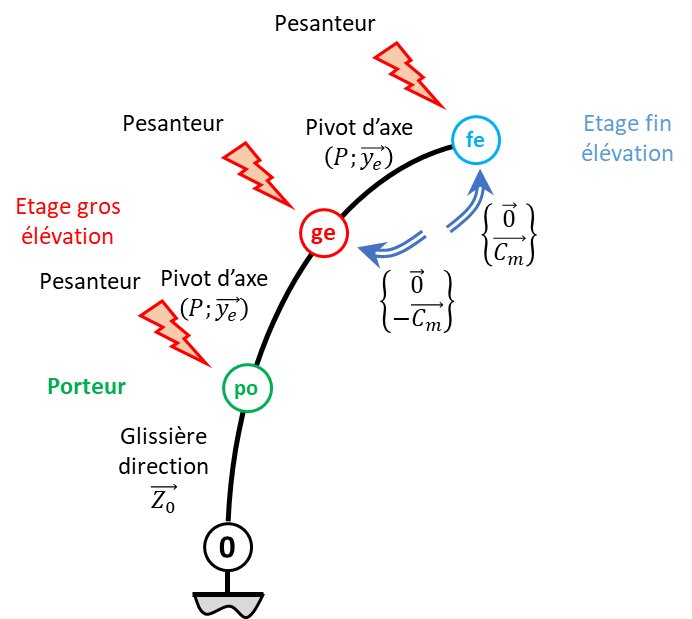
\includegraphics[width=\linewidth]{cor_11}
\end{center}
\end{minipage}\hfill
\begin{minipage}[c]{.6\linewidth}
\begin{itemize}
\item BAME : 
\begin{itemize}
\item pivot : $\torseurstat{T}{\text{ge}}{\text{fe}} = \torseurl{X\vect{x_e}+Y\vect{y_e}+Z\vect{z_e}}{L\vect{x_e}+N\vect{z_e}}{P}$;
\item couple moteur : $\torseurstat{T}{\text{mot}}{\text{fe}} = \torseurl{\vect{0}}{C_m(t)\vect{y_e}}{P}$;
\item pesanteur : $\torseurstat{T}{\text{pes}}{\text{fe}} = \torseurl{-\indice{m}{fe}g\vect{Z_0}}{\vect{0}}{\indice{G}{fe}}$. De plus, 
$\vectm{P}{\text{pes}}{\text{fe}} = \vect{0} + \vect{P\indice{G}{fe}}\wedge -\indice{m}{fe}g\vect{Z_0} =  \dfrac{m_od}{m_o+\indice{m}{cyl}}\vect{x_e} \wedge -\indice{m}{fe}g\vect{Z_0} $  $= \dfrac{m_od}{m_o+\indice{m}{cyl}}\indice{m}{fe}g\cos\theta \vect{ye} $
\end{itemize}
\end{itemize}
\end{minipage}

\begin{itemize}
\item Détermination du torseur dynamique en $\indice{G}{fe}$
\end{itemize}

Calcul de la résultante : $\vectrd{G}{fe}{\rep{0}} =m_{fe}\deriv{\vectv{G}{fe}{\rep{0}}}{\rep{0}}$ 

$ = m_{fe}\left(
 \dot{v}(t)\vect{Z_0}
-\thetapp_{\text{ea}}(t) \dfrac{m_o d}{m_o+\indice{m}{cyl}} \left(\sin\theta_{eo}\vect{X_0}+\cos\theta_{eo}\vect{Z_0} \right)
-\thetap^2_{\text{ea}}(t) \dfrac{m_o d}{m_o+\indice{m}{cyl}} \left(\cos\theta_{eo}\vect{X_0}-\sin\theta_{eo}\vect{Z_0} \right)\right)$ 


$ = m_{fe}\left(
 \dot{v}(t)\vect{Z_0}
-\thetapp_{\text{ea}}(t) \dfrac{m_o d}{m_o+\indice{m}{cyl}}\vect{z_e}
-\thetap^2_{\text{ea}}(t) \dfrac{m_o d}{m_o+\indice{m}{cyl}}\vect{x_e}\right)
$ 


%Calcul du moment : on calcul le moment dynamique en $G$ et on déplace en P :
%$\vectmc{\indice{G}{fe}}{fe}{\rep{0}} = \inertie{\indice{G}{fe}}{fe} \vecto{fe}{\rep0}$

Calcul du moment dynamique : la matrice d'inertie a été calculée en $P$. Faisons donc le calcul en $P$, point quelconque.

Calcul du moment cinétique en un point quelconque : 

$\vectmc{\indice{P}{fe}}{fe}{\rep{0}}= \inertie{\indice{P}{fe}}{fe} \vecto{fe}{\rep0} +\indice{m}{fe} \vect{P\indice{G}{fe}} \wedge \vectv{P}{}{\rep0}$
$=\inertie{\indice{P}{fe}}{fe} \thetap \vect{y_e} +\indice{m}{fe} \dfrac{m_od}{m_o+\indice{m}{cyl}}\vect{x_e} \wedge {v}\vect{Z_0} $
$ =\left( \indice{B}{cyl}+B_o+m_od^2\right) \thetap \vect{y_e}  + \indice{m}{fe} \dfrac{m_od}{m_o+\indice{m}{cyl}} {v} (-\cos \theta) \vect{y_e}$.

Calcul du moment dynamique en un point quelconque : 

$\vectmd{\indice{P}{fe}}{fe}{\rep{0}}= \deriv{\vectmc{\indice{P}{fe}}{fe}{\rep{0}}}{\rep{0}} + \vectv{P}{}{\rep{0}}\wedge  \indice{m}{fe}\vectv{G_{fe}}{fe}{\rep{0}} $
 
$ =\left( \indice{B}{cyl}+B_o+m_od^2\right) \thetapp \vect{y_e}  + \indice{m}{fe} \dfrac{m_od}{m_o+\indice{m}{cyl}} \left( -\dot{v} \cos \theta+{v} \thetap \sin \theta \right) \vect{y_e}
+  \indice{m}{fe} {v}\vect{Z_0}\wedge \left( v(t)\vect{Z_0}-\thetap_{\text{ea}}(t) \dfrac{m_o d}{m_o+\indice{m}{cyl}} \vect{z_e} \right) $ 

$ =\left( \indice{B}{cyl}+B_o+m_od^2\right) \thetapp \vect{y_e}  + \indice{m}{fe} \dfrac{m_od}{m_o+\indice{m}{cyl}} \left( -\dot{v} \cos \theta+{v} \thetap \sin \theta \right) \vect{y_e}
+  \indice{m}{fe} \dot{v}\left( -\thetap_{\text{ea}}(t) \dfrac{m_o d}{m_o+\indice{m}{cyl}}  \right) \sin\theta\vect{y_e} $

$ =\left( \indice{B}{cyl}+B_o+m_od^2\right) \thetapp \vect{y_e}  - \indice{m}{fe} \dfrac{m_od}{m_o+\indice{m}{cyl}} \dot{v} \cos \theta  \vect{y_e}
$


En appliquant le théorème du moment dynamique au solide $\text{fe}$ au point $P$ en projection sur  $\vect{y_e}$, on a donc : 

$$
\left( \indice{B}{cyl}+B_o+m_od^2\right) \thetapp  - \indice{m}{fe} \dfrac{m_od}{m_o+\indice{m}{cyl}} \dot{v} \cos \theta 
=  \dfrac{m_od}{m_o+\indice{m}{cyl}}\indice{m}{fe}g\cos\theta .
$$
\end{corrige}
\else
\fi

% Q12
\question{}
\ifprof
\begin{corrige}
Le couple perturbateur dû au déport de masse contient le terme de gravité ainsi que le terme d'accélération soit 
$\indice{C}{pert} = \gamma(t) m_o d \cos\theta_{eo}+m_o d g \cos\theta_{eo}$.

Les conditions les plus défavorables sont quant le terme en cosinus vaut 1 soit après application numérique :
$\indice{C}{pert} = 1,4 \times 0,01 \times 9,81 \times (1+1,8) \simeq \SI{0,385}{Nm}$.

Cela reste de l'ordre du dixième du couple moteur  proposé ($\simeq{3}{Nm}$), on peut donc le considérer comme négligeable.
\end{corrige}
\else
\fi

%Q13
\question{}
\ifprof
\begin{corrige}
$\vectv{A}{\text{fe}}{\rep{0}} =
\vectv{G_{\text{fe}}}{\text{fe}}{\rep{0}} \wedge \vect{G_{\text{fe}} A} = v(t) \vect{Z_0} + r\thetap_{\text{feo}}\vect{z_e}$ avec $\vect{AP}=\vect{AG_{\text{fe}}} = r\vect{x_e}$.

Or par composition de mouvement  
$\vectv{A}{\text{fe}}{\rep{0}}=
\vectv{A}{\text{fe}}{\text{ge}} +\vectv{A}{\text{ge}}{\rep{0}} $ ce qui conduit à la relation  $\indice{v}{tige}(t)=r\thetap_{\text{feo}}$.
\end{corrige}
\else
\fi

%Q14
\question{}
\ifprof
\begin{corrige}
On applique le principe fondamental de la dynamique à l'étage fin d'élévation et on écrit l'équation du moment dynamique au point $P$ 
(qui est considéré dans ce cas comme le centre d'inertie). 
Par rapport au calcul précédent le couple moteur est remplacé par le moment de l'action du moteur linéaire soit  $r\indice{F}{mot} \vect{y_e}$, 
le moment de la pesanteur est nul en $P$ et celui de l'action de la liaison pivot parfaite aussi. 
Cela conduit à  
$\vectmd{P}{fe}{\rep{0}}=r\indice{F}{mot} \vect{y_e}$.  
Or le point $P$ étant le centre d'inertie, le moment dynamique est directement égal à la dérivée du moment cinétique exprimé en ce même point soit  $\vectmd{P}{fe}{\rep{0}} = \indice{B}{fe}\thetapp_{\text{feo}}=r\indice{F}{mot}$.
L'équation du mouvement se réduit à  $\indice{B}{fe}\thetapp_{\text{feo}}=r\indice{F}{mot}$. On passe cette expression dans le domaine de Laplace (en considérant les conditions initiales nulles) ce qui conduit à : $\indice{B}{fe} p^2 \theta_{\text{feo}}(p)=r\indice{F}{mot}(p)$ 
 d'où la fonction de transfert recherchée :  $\dfrac{\indice{\Omega}{fe}(p)}{\indice{F}{mot}(p)} = \dfrac{r}{\indice{B}{fe} p}$.

La lecture du schéma bloc proposé permet d'écrire   $\dfrac{\indice{\Omega}{fe}(p)}{\indice{F}{mot}(p)} = \dfrac{K_1}{M_{\text{eq}} p}$  soit par identification (en prenant garde aux dimensions)  $K_1 = \dfrac{1}{r}$ (\si{m^{-1}}) et  $\indice{M}{eq} = \dfrac{\indice{B}{fe}}{r^2}$ (\si{kg}).


\end{corrige}
\else
\fi

% Q15
\question{}
\ifprof
\begin{corrige}
Le gyromètre étant modélisé par une fonction transfert d'ordre 1 et de gain 1, on a directement $\dfrac{1}{\indice{\tau}{gyro}}={2\pi f}$ soit $\indice{\tau}{gyro} = \dfrac{1}{2 \pi 100} \simeq \SI{1,6}{ms}$.
\end{corrige}
\else
\fi

% Q16
\question{}
\ifprof
\begin{corrige}
On a d'une part, 
$F(p) = \dfrac{\dfrac{\indice{K}{fe}}{\indice{R}{fe}\indice{M}{eq}p}}{1+\dfrac{\indice{K}{fe}}{\indice{R}{fe}\indice{M}{eq}p}\indice{K}{fe}}$
$= \dfrac{\indice{K}{fe}}{\indice{R}{fe}\indice{M}{eq}p+ \indice{K}{fe}^2}$


D'autre part, 
$\indice{H}{fe} (p)= \dfrac{\indice{H}{corfe}(p) F(p) K_1 }{1+\indice{H}{corfe}(p)\indice{H}{gyro}(p) F(p) K_1 }$
$ = \dfrac{\indice{H}{corfe}(p) \dfrac{\indice{K}{fe}}{\indice{R}{fe}\indice{M}{eq}p+ \indice{K}{fe}^2} K_1 }{1+\indice{H}{corfe}(p)\indice{H}{gyro}(p) \dfrac{\indice{K}{fe}}{\indice{R}{fe}\indice{M}{eq}p+ \indice{K}{fe}^2} K_1 }$ 


$ = \dfrac{\indice{H}{corfe}(p) \indice{K}{fe} K_1 }{\indice{R}{fe}\indice{M}{eq}p+ \indice{K}{fe}^2+\indice{H}{corfe}(p)\indice{H}{gyro}(p) \indice{K}{fe} K_1} $ 
$ = \dfrac{\indice{H}{corfe}(p) \indice{K}{fe} K_1 }{\indice{R}{fe}\indice{M}{eq}p+ \indice{K}{fe}^2+\indice{H}{corfe}(p)\dfrac{1}{1+\indice{\tau}{gyro}p}\indice{K}{fe} K_1} $ 

$ = \dfrac{\indice{H}{corfe}(p) \indice{K}{fe} K_1 \left(1+\indice{\tau}{gyro}p\right)}{ \left(1+\indice{\tau}{gyro}p\right) \indice{R}{fe}\indice{M}{eq}p+  \left(1+\indice{\tau}{gyro}p\right) \indice{K}{fe}^2+\indice{H}{corfe}(p)\indice{K}{fe} K_1} $.

Avec $\indice{H}{corfe}(p) = 1$, 
$ \indice{H}{fe} (p) = \dfrac{ \indice{K}{fe} K_1 \left(1+\indice{\tau}{gyro}p\right)}{ \left(1+\indice{\tau}{gyro}p\right) \indice{R}{fe}\indice{M}{eq}p+  \left(1+\indice{\tau}{gyro}p\right) \indice{K}{fe}^2+\indice{K}{fe} K_1} $ 

$ = \dfrac{ \dfrac{\indice{K}{fe} K_1}{\indice{K}{fe} K_1+\indice{K}{fe}^2} \left(1+\indice{\tau}{gyro}p\right)}{ \dfrac{\left(1+\indice{\tau}{gyro}p\right)}{\indice{K}{fe} K_1+\indice{K}{fe}^2} \indice{R}{fe}\indice{M}{eq}p+  \indice{\tau}{gyro}p\dfrac{ \indice{K}{fe}^2}{\indice{K}{fe} K_1+\indice{K}{fe}^2}+1} $ 
$ = \dfrac{ K_1}{ K_1+\indice{K}{fe}} \dfrac{ 1+\indice{\tau}{gyro}p}{ \dfrac{\indice{\tau}{gyro} \indice{R}{fe}\indice{M}{eq} }{\indice{K}{fe} K_1+\indice{K}{fe}^2} p^2+  p\dfrac{ \indice{R}{fe}\indice{M}{eq}+\indice{\tau}{gyro}\indice{K}{fe}^2}{\indice{K}{fe} K_1+\indice{K}{fe}^2}+1} $. 

\end{corrige}

\else
\fi

%Q17
\question{}
\ifprof
\begin{corrige}
D'après la fonction de transfert proposée, on peut déterminer la pulsation propre non amortie du 
système $\omega_0 = \sqrt{\dfrac{1}{6\times 10^{-4}}}\simeq \SI{40,825}{rad.s^{-1}}$
et l'amortissement $\xi=\dfrac{\omega_0}{2} \times 3,65 \times 10^{-1} \simeq 7,45$.

Ce qui à l'aide de l'abaque permet de déterminer le temps de réponse réduit $t_{5\%} \omega_0= 45$ 
d'où  $t_{5\%} \simeq \dfrac{45}{40,825}\simeq \SI{1,1}{s}$. Le critère du temps de réponse de $<\SI{40}{ms}$ n'est pas respecté. De plus 
l'écart statique vaut $1-0,5\times 1=0,5 \neq 0$ ce qui ne respecte pas le cahier des charges.
\end{corrige}
\else
\fi


%Q18
\question{}
\ifprof
\begin{corrige}~\\
\begin{center}

\includegraphics[width=.7\linewidth]{cor_18}
\end{center}

\begin{center}
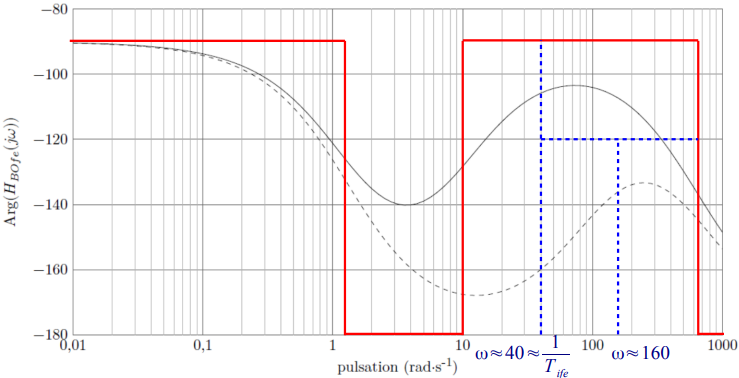
\includegraphics[width=.7\linewidth]{cor_18_bode}
\end{center}
\end{corrige}
\else
\fi


%Q19
\question{}
\ifprof
\begin{corrige}
On a $\varphi(\omega)=-90 +\arctan \left( T_{ife} \omega \right)-\arctan \left( 0,75 \omega \right)-\arctan \left( 1,6\times 10^{-3} \omega \right)$.

Entre 10 et 600 \si{rad/s}, la phase associée à $\dfrac{1}{1+0,75p}$ tend vers $-90\degres$.

On cherche alors $\omega$ tel que $\varphi(\omega) = -120\degres$ soit 
$-90 +\arctan \left( T_{ife} \omega \right)-90-\arctan \left( 1,6\times 10^{-3} \omega \right) = -120 $ et  
$\arctan \left( T_{ife} \omega \right)-\arctan \left( 1,6\times 10^{-3} \omega \right) = 60 $.
En passant à la tangente,
$ \dfrac{ T_{ife} \omega - 1,6\times 10^{-3} \omega }{1+ T_{ife} \omega \times 1,6\times 10^{-3} \omega } = \tan 60$
soit 
$  T_{ife} \omega - 1,6\times 10^{-3} \omega = \tan 60+ \tan 60 T_{ife} \omega \times 1,6\times 10^{-3} \omega $
puis
$    27,7\times 10^{-5} \omega^2 -  0,0984 \omega  - \tan 60 = 0$.


On a alors $\Delta= 0,0116$ et $\omega = \dfrac{0,0984\pm 0,198}{0,000554}\simeq \SI{535}{rad/s}$

\end{corrige}
\else
\fi


%Q20
\question{}
\ifprof
\begin{corrige}
Pour une marge de phase de 60\degres, il faut que la pulsation pour laquelle le gain s'annule soit celle 
pour laquelle la phase vaut -120\degres. La lecture graphique donne $\omega \simeq \SI{160}{rad/s}$
 et à cette 
pulsation le gain harmonique vaut $\simeq -\SI{43}{dB}$. Il faut donc réaliser une translation de la courbe 
de gain pour l'annuler à cette valeur de pulsation, soit $20\log \indice{K}{pfe}=\SI{43}{dB}$ ce qui donne
$\indice{K}{pfe}=141,3$.
\end{corrige}
\else
\fi


%Q21
\question{}
\ifprof
\begin{corrige}
La figure permet de voir que la tension d'alimentation du moteur a été saturée pendant une durée 
de 25(ms) environ, soit presque 2 fois plus que ce la commande aurait exigé. Pendant cette durée le 
moteur n'est plus en régime asservi mais fonctionne en tout ou rien. Le fait d'avoir prolongé cette 
durée de saturation de 13(ms) à 25 (ms) permet de limiter le dépassement et de ce fait de diminuer 
le temps de réponse du système.
 
Le correcteur ayant par ailleurs annulé l'erreur statique et assuré la marge de phase, les contraintes 
du cahier des charges sont respectées : temps de réponse, marge de phase, erreur statique.

\end{corrige}
\else
\fi


%Q22
\question{}
\ifprof
\begin{corrige}
Le signal de consigne peut être représenté temporellement par trois signaux de type « rampe » :
\begin{itemize}
\item rampe 1 de pente $a=\dfrac{\pi}{0,26} \si{rad.s^{-2}}$ retardée de $\simeq \SI{0,71}{s}$ (par lecture graphique);
\item rampe 2 de pente $-2a$ retardée de $\simeq \SI{0,71}{s}+\SI{0,26}{s}$;
\item rampe 3 de pente $a$ retardée de  $\simeq \SI{0,71}{s}+2\times \SI{0,26}{s}$.
\end{itemize}
De ce fait le signal de consigne en position est constitué de branches de parabole avec un changement de concavité pour $t\simeq \SI{0,97}{s}$ et une valeur maximale obtenue pour  $\simeq \SI{0,82}{rad}$.

\begin{center}
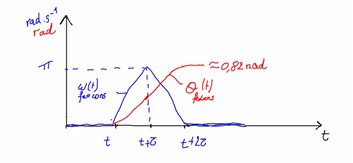
\includegraphics[width=3cm]{cor_22}
\end{center}

\end{corrige}
\else
\fi


%Q23
\question{}
\ifprof
\begin{corrige}
Le signal en rampe permet d'évaluer le retard de traînage, la consigne finale l'erreur statique donc la
précision angulaire de positionnement et les éventuelles oscillations la stabilité de la ligne de visée.

Tous les critères sont donc évaluables avec cette entrée. 

\end{corrige}
\else
\fi


%Q24
\question{}
\ifprof
\begin{corrige}
Dans le graphe ci-dessous, on constae que $\beta(t)_{\text{max}} \simeq \SI{0,08}{rad}$ or géométriquement on observe que l'angle $\angl{{u}}{{z_e}} <\angl{{z_{ge}}}{{z_e}}$
soit $\angl{{u}}{{z_e}}<\beta(t)$. On peut donc conclure que $\vect{u}\simeq \vect{z_e}$ est justifiée.

\begin{center}
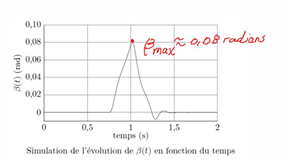
\includegraphics[width=3cm]{cor_24_01}
\end{center}
On peut lire sur le graphe : 
\begin{itemize}
\item le retard de traônage d'une valeur nettement inférieure à \SI{40}{ms} du cahier des charges : critère satisfait;
\item l'erreur qui est nulle : critère de précision satisfait;
\item le dépassement de \SI{3}{mrad} : critère non satisfait (\SI{340}{\mu rad} dans le cahier des charges). 
\end{itemize}
\begin{center}
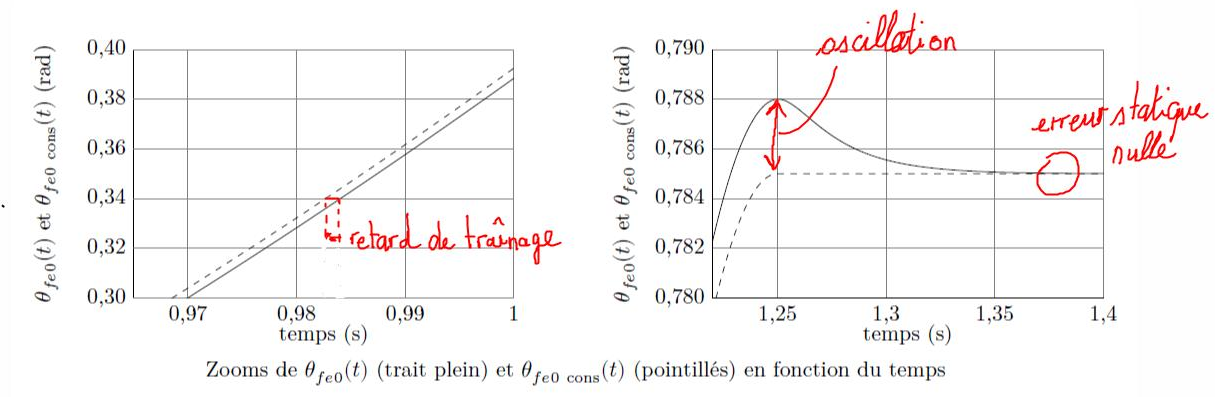
\includegraphics[width=6cm]{cor_24_02}
\end{center}

\end{corrige}
\else
\fi

%
%
%\begin{figure}[H]
%\centering
%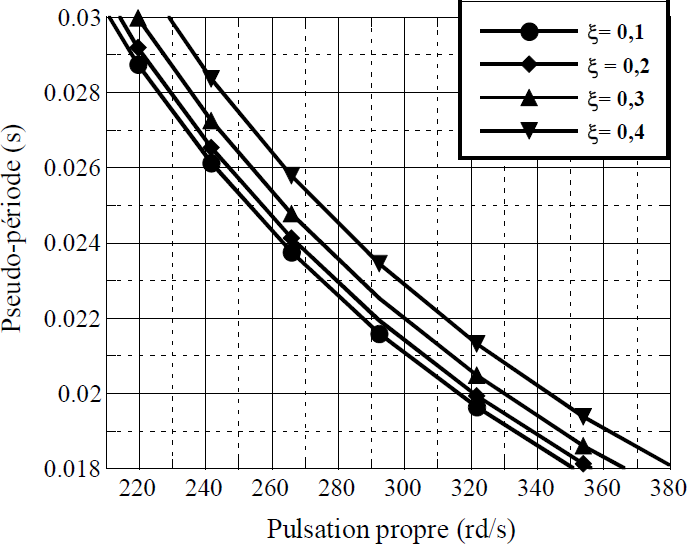
\includegraphics[width=.8\linewidth]{fig_14}
%\caption{\label{fig:14}  }
%\end{figure}


\end{document}



